The Google Android operating system was chosen as the client platform. This
decision was based primarily on two factors, firstly that the teams mobile
development experience was mainly with Android and additionally the
availability of development hardware for the duration of the project.

As a part of our white-boarding meetings, we developed a high level idea of the
functionality required by the client interface this can be seen in
Figure~\ref{fig:system_components}.

To create a structure for the client the team explored a number of low fidelity
user interface options. The agreed upon interface was used as a basis to create
an architecture for the project. The identified components and their
communications are described in Figure~\ref{fig:client_design}.

\begin{figure}[htb]
\centering
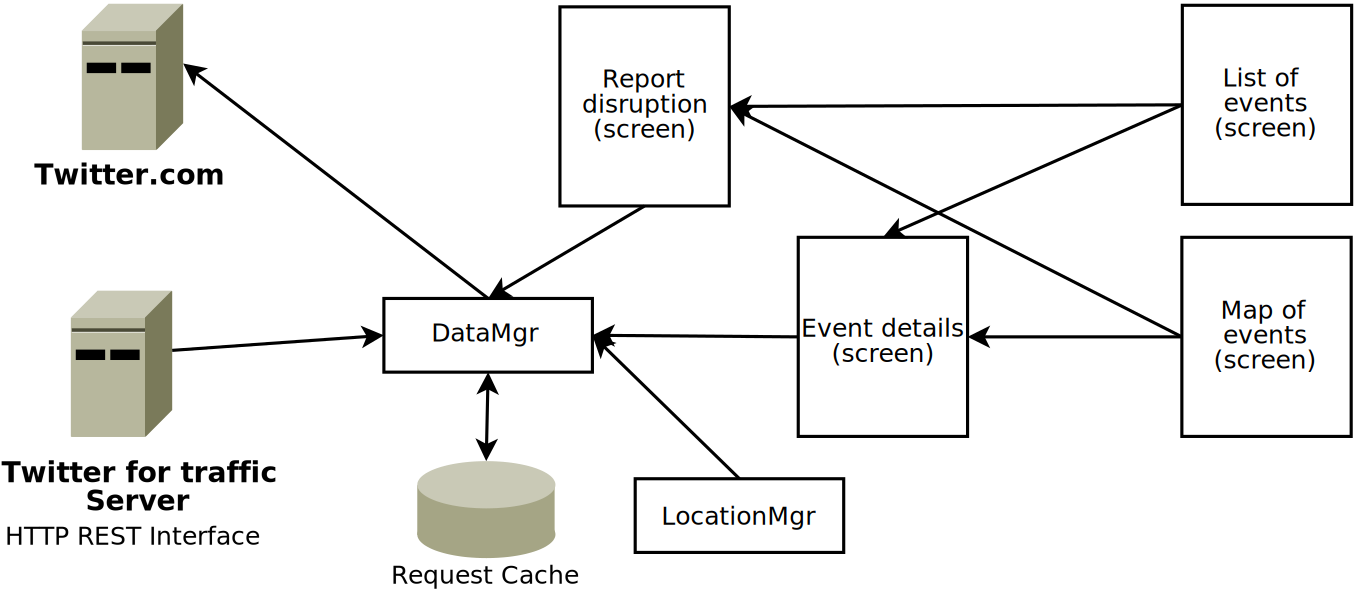
\includegraphics[width=0.9\textwidth]{images/design/client/client_high_level_layout.pdf}
\caption{High level client design}
\label{fig:client_design}
\end{figure}



\subsubsection{User interface}
\subsubsection{Request caching}
